\documentclass{beamer}

\usepackage[francais]{babel}
\usepackage[utf8]{inputenc}
\usepackage[T1]{fontenc}
\usepackage{graphicx}
\usepackage{graphics}
\usepackage{color}
\usepackage{textcomp}
\usepackage{pifont}
\usepackage[normalem]{ulem}
\usepackage{times}
\usepackage{hyperref}
\usepackage{verbatim}
\usepackage{amsmath}
\usepackage{amsthm}
\usepackage{amsfonts}
\usepackage[mathscr]{euscript}
\usepackage{pgfpages}
\usepackage{listings}
\usepackage{subfigure}
\usepackage{algorithm}
\usepackage[noend]{algorithmic}
\usepackage{pdftricks}
\usepackage{mathrsfs}
\usepackage{array}
\usepackage{fancybox}
% \usepackage{columns}
\usepackage{multirow}
\usepackage{url}
\usepackage{tikz}
\usepackage{colortbl}
%\usepackage{cite} %DO NOT FUCKING USE CITE ON BEAMER !!! LOST 30 GODDAM' MINUTES ON THIS SHIT !!!
\usepackage{mathabx}
\usepackage{amssymb}
\usepackage{eurosym}
\usepackage{wasysym} % ch0

\let\texteuro\euro

\hypersetup{colorlinks,%
            citecolor=black,%
            filecolor=black,%
            linkcolor=black,%
            urlcolor=blue}

%\addtolength{\parskip}{10pt}

\usetikzlibrary{calc}

\mode<presentation>
\setbeamertemplate{footline}[frame number]
\setbeamercovered{transparent}
\usetheme[navigation]{ESI}

%lst
\definecolor{comment-green}{RGB}{0,166,80}
\lstset{language=C++,
  keywordstyle=\lst@ifdisplaystyle\bf\fi\color{blue!60},
  commentstyle=\color{comment-green},
  stringstyle=\color{red},
  basicstyle=\lst@ifdisplaystyle\tiny\else\tt\fi,
  morekeywords={
    constexpr,concept,decltype,nullptr,nullptr_t,noexcept,final,override},
  frame=single,
  xleftmargin=0.5cm,
  numbers=left,
  tabsize=2}

%title
\subtitle{Langage \texttt{C} / \cpp}
\author{R. Absil}
\date{\today}

%styles
\theoremstyle{definition}
\newtheorem{thm}{Théorème}
\newtheorem{conj}[thm]{Conjecture}
\newtheorem{deff}[thm]{Définition}
\newtheorem{prop}[thm]{Propriété}
\newtheorem{lem}[thm]{Lemme}
\newtheorem*{lem*}{Lemme}
\newtheorem{cor}[thm]{Corollaire}
%\newtheorem{example}{Exemple}
\newtheorem{remark}{Remarque}
\newtheorem{exo}{Exercice}

%typeset
\newcommand{\ie}{{\emph{i.e., }}}
\newcommand{\eg}{{\emph{e.g., }}}
\newcommand{\etal}{{\emph{et al.}}}
\newcommand{\rrceil}{\unichar{"2308}}
\newcommand{\sloand}[2]{\footnote{N. J. A. Sloane - OEIS Foundation - \texttt{www.oeis.org}, Sequence #1 - #2.}}

%math
\newcommand{\IN}{{\mathbb N}}
\newcommand{\IQ}{{\mathbb Q}}
\newcommand{\IR}{{\mathbb R}}
\newcommand{\IZ}{{\mathbb Z}}
\newcommand{\IP}{{\mathbb P}}
\newcommand{\IC}{{\mathbb C}}
\newcommand{\bigo}{{\mathcal{O}}}
\renewcommand{\mod}{\bmod}
\newcommand{\ssi}{\Leftrightarrow}
\newcommand{\then}{\Rightarrow}
\newcommand{\fle}[1]{\stackrel{#1}{\longrightarrow}}
\newcommand{\suchthat}{~\big|~}
\newcommand{\floor}[1]{\left\lfloor #1 \right\rfloor}
\newcommand{\ceil}[1]{\left\lceil #1 \right\rceil}
\DeclareMathOperator*{\argmin}{argmin}
\DeclareMathOperator*{\argmax}{argmax}

%tikz
\tikzstyle{_vertex}=[fill=white, circle,minimum size=12pt,inner sep=1pt]
\tikzstyle{_blackv}=[fill=black, circle,minimum size=8pt,inner sep=1pt]
\tikzstyle{_dot}=[fill=black, circle, minimum size = 1mm, inner sep=0pt]
\tikzstyle{_bigvertex}=[fill=white, circle,minimum size=21pt,inner sep=1pt]
\tikzstyle{_arc}=[->, >=stealth]
\tikzstyle{_boldarc}=[->, >=stealth, line width=2pt]

\newcommand{\cpp}{\texttt{C++}}
\newcommand{\java}{\texttt{Java}}


\title{Ch. 1 - Concepts de base}

\begin{document}
\begin{frame}
  \titlepage
\end{frame}

\begin{frame}
  \frametitle{Table des matières}
  \footnotesize \tableofcontents[pausesections,pausesubsections]
\end{frame}


\section{Introduction}

\begin{frame}
\frametitle{Différences majeures entre \java\ et \texttt{C} / \cpp}
\begin{itemize}[<+->]
\item La sortie du compilateur est un fichier binaire directement exécuté par le processeur
\item \emph{Tout} est passé par valeur, en l'absence de spécifications explicites
\item Un \lstinline|new| en \cpp\ (ou son équivalent en \texttt{C}) est significativement plus difficile à gérer
	\begin{itemize}
	\item Mais de bonnes pratiques permettent d'éviter les ennuis
	\end{itemize}
\item Une plus grande liberté de programmation en \cpp
	\begin{itemize}
	\item Surcharge d'opérateur
	\item Conversions définies par l'utilisateur
	\item Une bonne hygiène de programmation est nécessaire
	\end{itemize}
\item Le polymorphisme n'est pas «~activé~» par défaut
\item Pas de franches relations d'héritage entre classes aux fonctionnalités «~similaires~»
\item Mécanisme de types génériques implémenté à la compilation
\end{itemize}
\end{frame}


\begin{frame}
\frametitle{Différences \texttt{C} et \cpp}
\begin{itemize}[<+->]
\item \texttt{C} : Langage procédural uniquement.
	\begin{itemize}
	\item Pas d'orienté objet et concepts associés.
%	\item Fonctionnel limité (pas de surcharge de \texttt{()})
	\end{itemize}
\item Pas de surdéfinition de fonctions
\item Pas d'inférence de type.
\item Pas de surcharge d'opérateur.
\item Pas de références.
\item Pas d'exceptions.
\item Pas de patrons.
\item Pas d'espaces de noms.
\item Pas de conversions définies par l'utilisateur.
\item Pas de conteneurs standards.
\item Pas de \texttt{string}
\end{itemize}
\end{frame}

\begin{frame}
\frametitle{Concepts inexistants en \texttt{C}}
\begin{center}
\begin{footnotesize}
\textcolor{blue!60}{
\begin{tabular}{llll}
\texttt{try} & \texttt{catch} & \texttt{throw} & \texttt{typeid}\\
\texttt{const\_cast} & \texttt{dynamic\_cast} & \texttt{reinterpret\_cast} & \texttt{static\_cast}\\
\texttt{namespace} & \texttt{friend} & \texttt{operator} & \texttt{mutable}\\
\texttt{template} &\texttt{typename} & \texttt{new} & \texttt{delete}\\
\texttt{protected} & \texttt{public} & \texttt{private} & \texttt{class}\\
\texttt{this} & \texttt{explicit} & \texttt{using} & \texttt{virtual}\\
\texttt{export} & \texttt{concept}\\
\end{tabular}}
\end{footnotesize}
\end{center}
\end{frame}

\begin{frame}[containsverbatim]
\frametitle{\texttt{C} : le programme minimal}
\begin{itemize}
\item Fichier \texttt{hello-world.c}
\end{itemize}
\begin{lstlisting}
#include <stdio.h>

int main() //variantes avec arguments en ligne de commande
{
	printf("Hello World!\n");
}
\end{lstlisting}
\begin{itemize}
\item \lstinline|#include| permet d'importer les fichiers nécessaires
\item La fonction \lstinline|int main()| est l'unique point d'entrée du programme
\item \texttt{printf} est une fonction permettant d'imprimer en console
	\begin{itemize}
	\item On peut spécifier des «~formats~» pour formater l'affichage
	\end{itemize}
\item Syntaxe de commentaires comme en \java
\item Compilation avec \texttt{gcc -o sortie monficher.c}
\end{itemize}
\end{frame}

\section{Compilation}

\begin{frame}
\frametitle{Production d'un exécutable en trois temps}
\begin{enumerate}[<+->]
\item Précompilation
	\begin{itemize}
	\item Directives précédées de \texttt{\#} (préprocesseur)
		\begin{itemize}
		\item Inclusions des fichiers d'entête		
		\end{itemize}
	\item Immédiats convertis en numériques, etc.
	\item Produit un programme en \texttt{C} / \cpp\ pur
	\item Sortie : fichier texte
	\end{itemize}
\item Compilation
	\begin{itemize}
	\item Analyse lexicale, syntaxique et sémantique
	\item Traduction du programme en langage machine
	\item Produit des fichiers objets
	\end{itemize}
\item Édition des liens
	\begin{itemize}
	\item Lie les références et appels entre eux
	\item Ajoute les librairies externes
	\item Produit un fichier exécutable ou une librairie directement utilisable
	\end{itemize}
\end{enumerate}
\end{frame}

\begin{frame}[containsverbatim]
\frametitle{Illustration préprocesseur}
\begin{itemize}
\item Fichier \texttt{preproc.c}
\end{itemize}
\begin{lstlisting}
... 

extern int printf (const char *__restrict __format, ...);

...

int main()
{
	printf("Hello World!\n");
}
\end{lstlisting}
\begin{itemize}
\item Obtenu avec \texttt{gcc -E hello-world.c}
\item Assembleur obtenu avec \texttt{-S}
	\begin{itemize}
	\item Fichier \texttt{hello-world.s}
	\end{itemize}
\end{itemize}
\end{frame}

\begin{frame}
\frametitle{Compilation séquentielle}
\begin{itemize}[<+->]
\item En \texttt{C} / \cpp, un programme est lu séquentiellement de haut en bas
	\begin{itemize}
	\item L'ordre des déclarations importe
	\end{itemize}
\item Motive l'usage des headers
	\begin{itemize}
	\item On déclare une fois pour tout le programme
	\item On ne veut pas inclure deux fois un header
	\end{itemize}
\item Les headers ne sont pas «~compilés directement~» : ils sont inclus (copier / coller textuel) à l'étape de précompilation
\item Peut poser problème en cas de dépendances cycliques
	\begin{itemize}
	\item Usage d'instructions de compilation conditionnelles
	\item Usage de pointeurs pour éviter une taille infinie (cf. Ch. 2)
	\end{itemize}
\item Point d'entrée : \texttt{main}
\item Options de compilations additionnelles
	\begin{itemize}
	\item \texttt{-Wpedantic}, \texttt{-o3},\texttt{-fno-stack-protector}, \texttt{-l}, etc.
	\end{itemize}
\end{itemize}
\end{frame}

\begin{frame}[containsverbatim]
\frametitle{Exemple : ordre importe}
\begin{itemize}
\item Fichier \texttt{order.c}
\end{itemize}
\begin{lstlisting}
void g();

int main()
{
	f();
	g();
}

void f()
{
	printf("Coucou");
}

void g()
{
	printf("Beuh");
}
\end{lstlisting}
\end{frame}

\begin{frame}[containsverbatim]
\frametitle{Exemple : inclusion multiple}
\begin{itemize}
\item Fichier \texttt{incl-mult.c}
\end{itemize}
\begin{lstlisting}
#include <stdio.h>
#include "incl-mult2.c"

void g()
{
	printf("Beuh\n");
}

int main()
{
	f();
}
\end{lstlisting}
\begin{itemize}
\item Fichier \texttt{incl-mult2.c}
\end{itemize}
\begin{lstlisting}
#include <stdio.h>
#include "incl-mult.c"

void f()
{
	printf("Coucou\n");
	g();
}

\end{lstlisting}
\begin{itemize}
\item Solutions : \texttt{incl-mult-fixed*}
\end{itemize}
\end{frame}

\begin{frame}[containsverbatim]
\frametitle{Solution}
\begin{itemize}
\item Séparer les déclarations et leur implémentation
\item Utiliser \lstinline|#ifndef| / \lstinline|#define|
\end{itemize}
\begin{lstlisting}
#ifndef MULT_1
#define MULT_1
	void g();
#endif
\end{lstlisting}
\begin{lstlisting}
#ifndef MULT_2
#define MULT_2
	void f();
#endif
\end{lstlisting}
\begin{lstlisting}
#include "incl-mult-fixed.h"
#include "incl-mult-fixed-2.h"

int main()
{
	f();
	g();
}
\end{lstlisting}
\begin{itemize}
\item On met les \lstinline|#include| là où il le faut
\end{itemize}
\end{frame}

\section{Types de base}

\begin{frame}
\frametitle{Notion de type (1/2)}
\begin{itemize}[<+->]
\item Définit le codage en mémoire
\item Définit à quoi correspond un motif
\end{itemize}
\begin{exampleblock}<+->{Exemple}
	\begin{itemize}[<+->]
	\item Motif binaire \texttt{010011001}
		\begin{itemize}
		\item Nombre $77$
		\item Adresse \texttt{0x4D}
		\item Caractère ASCII 'M'
		\end{itemize}
	\end{itemize}
\end{exampleblock}
\end{frame}

\begin{frame}
\frametitle{Notion de type (2/2)}
\begin{itemize}[<+->]
\item Deux sortes de types
	\begin{enumerate}
	\item Scalaire : contient une unique valeur à un moment donné
	\item Structuré : contient plusieurs valeurs
		\begin{itemize}
		\item Potentiellement de différents types
		\item Motif à découper
		\end{itemize}
	\end{enumerate}
\end{itemize}
\begin{exampleblock}<+->{Exemple}
	\begin{itemize}
	\item Scalaire : \lstinline|int|, \lstinline|double|, \lstinline|char|, \lstinline|float*|, \lstinline|enum|
	\item Structuré : tableaux, classes, structures \texttt{C}, \texttt{string} (\cpp), etc.
	\end{itemize}
\end{exampleblock}
\end{frame}

\begin{frame}
\frametitle{Type incomplet}
\begin{itemize}[<+->]
\item Dans une vaste majorité des cas, le compilateur requiert qu'un type $T$ soit \emph{complet}
	\begin{itemize}
	\item Si on a besoin de sa taille (pour allouer un $T$)
	\item Si on a besoin de connaître les opérations que l'on peut réaliser sur un $T$ (appel de fonction en \cpp)
	\end{itemize}
\item Les types suivants sont \emph{incomplets}
	\begin{itemize}
	\item \lstinline|void| et ses versions cv-qualifiées
	\item une classe déclarée mais non définie (forward declaration)
	\item un tableau de taille inconnue (avec \lstinline|extern|)
	\item un tableau d'éléments de types incomplets
	\end{itemize}
\item Parfois, certaines portions de code requièrent d'utiliser temporairement un type incomplet
	\begin{itemize}
	\item Par ex., dans le cadre d'inclusions multiples
	\end{itemize}
\end{itemize}
\end{frame}

\begin{frame}
\frametitle{Les types de base et le standard \texttt{C} /  \cpp}
\begin{itemize}[<+->]
\item Le standard \texttt{C} / \cpp\ impose peu de contraintes de taille
	\begin{itemize}
	\item Un \lstinline|int| sur une machine n'a peut-être pas la même taille qu'un \lstinline|int| sur une autre
	\end{itemize}
\item Contraintes de bornes pour les types numériques
	\begin{itemize}
	\item Un \lstinline|int| est généralement 32 bits, un \lstinline|double| sur 64 bits
	\item Bornes dans \texttt{limits.h}
	\end{itemize}
\item La représentation des négatifs n'est pas fixée
	\begin{itemize}
	\item Souvent, complément à deux, little indian
	\end{itemize}
\item La représentation des flottants n'est pas fixée
	\begin{itemize}
	\item Souvent, norme IEEE-754 64 bit
	\end{itemize}
\item Il convient de savoir avec quoi on travaille
\item Référence complète : \url{https://en.cppreference.com/w/c/language/arithmetic_types}
\end{itemize}
\end{frame}

\begin{frame}[containsverbatim]
\frametitle{Bornes}
\begin{itemize}
\item En \texttt{C} : fichier \texttt{bounds.c}
\item On imprime avec \texttt{printf} et en spécifiant un format (cf. section suivante)
\end{itemize}
\begin{lstlisting}
#include <stdio.h>
#include <limits.h>
#include <float.h>
 
int main(void)
{   
    printf("INT_MIN    = %+d\n", INT_MIN);
    printf("INT_MAX    = %+d\n", INT_MAX);
    printf("UINT_MAX   = %u\n",  UINT_MAX);
    printf("\n");
 
    printf("FLT_MIN    = %e\n", FLT_MIN);
    printf("FLT_MAX    = %e\n", FLT_MAX);
   	printf("\n");
   	
    printf("DBL_MIN    = %e\n", DBL_MIN);
    printf("DBL_MAX    = %e\n", DBL_MAX);
   	printf("\n");
}
\end{lstlisting}
\end{frame}

\begin{frame}
\frametitle{Ce que l'on sait des tailles}
\begin{itemize}[<+->]
\item \lstinline|sizeof(type)| permet de connaître la taille d'un type (en bytes)
	\begin{itemize}
	\item Ne peut être utilisé sur des fonctions ou des types incomplets
	\end{itemize}
\item Un byte est constitué de $8$ bits ou plus
	\begin{itemize}
	\item Généralement $8$
	\item Spécifié par \texttt{CHAR\_BIT}
	\end{itemize}
\item Un \lstinline|char| est toujours de taille $1$ (byte)
\item Une adresse (pointeur) est de la taille du bus d'adresse (32 bits en x86, 64 bits en x64)
\item La taille d'une classe ou structure est au moins la somme des tailles de ses attributs
	\begin{itemize}
	\item Mais pas toujours, dépendant des contraintes d'alignement
%	\item \lstinline|sizeof(T)| retourne la taille d'un élément d'un tableau de $T$
	\end{itemize}
\end{itemize}
\end{frame}

\begin{frame}[containsverbatim]
\frametitle{Taille des types de base}
\begin{itemize}
\item Fichier \texttt{sizeof.c}
\item En \cpp\ : même principe en imprimant avec \texttt{std::cout}
\end{itemize}
\begin{lstlisting}
#include "stdio.h"

int main()
{
	printf("Size of char             : %lu bytes\n", sizeof(char));
	printf("Size of short            : %lu bytes\n", sizeof(short));
	printf("Size of int              : %lu bytes\n", sizeof(int));
	printf("Size of long int         : %lu bytes\n", sizeof(long int));
	printf("Size of long long int    : %lu bytes\n", sizeof(long long int));
	printf("Size of adress           : %lu bytes\n", sizeof(int*));
	printf("Size of float            : %lu bytes\n", sizeof(float));
	printf("Size of double           : %lu bytes\n", sizeof(double));
	printf("Size of long double      : %lu bytes\n", sizeof(long double));
}
\end{lstlisting}
\end{frame}

\begin{frame}[containsverbatim]
\frametitle{Illustration}
\begin{itemize}
\item Fichier \texttt{align.c} (même principe en \cpp)
\end{itemize}
\begin{lstlisting}
struct A
{
	int i; //size 4
};

struct B
{
	char c; //size 1
};

struct C
{
	int i; //size 4
	char c; //size 1
	//3 bytes padding
}; //size 8

int main()
{
	printf("%lu %lu %lu\n", sizeof(struct A), sizeof(struct B), sizeof(struct C));
}
\end{lstlisting}
\end{frame}

\begin{frame}
\frametitle{Types entiers}
\begin{itemize}[<+->]
\item Différents types d'entiers
	\begin{itemize}
	\item \lstinline|short int| (abrégé en \lstinline|short|)
	\item \lstinline|int|
	\item \lstinline|long int| (abrégé en \lstinline|long|)
	\item \lstinline|long long int| (abrégé en \lstinline|long long|)
	\end{itemize}
\item Limites de codage différentes
\item Possibilité de travailler en non signé
	\begin{itemize}
	\item \lstinline|unsigned long int|
	\item Permet de doubler la valeur maximum du codage
	\item Mettre un négatif dans un \lstinline|unsigned| conduit à un comportement indéterminé
	\end{itemize}
\item Immédiats codé comme \texttt{1}, \texttt{017}, \texttt{0x1A}, etc.
\item Par défaut, les immédiats entiers sont de type \lstinline|int|
\item Type forcé via suffixes \texttt{u}, \texttt{l}, \texttt{ul}
	\begin{itemize}
	\item \texttt{3 + 42ul}
	\end{itemize}
\end{itemize}
\end{frame}

\begin{frame}[containsverbatim]
\frametitle{Illustration}
\begin{itemize}
\item Fichier \texttt{int.c} (même principe en \cpp)
\end{itemize}
\begin{lstlisting}
#include <stdio.h>
#include <limits.h>

int main()
{
	unsigned i = -1;
	if(i == UINT_MAX)
		printf("Two complement\n");
	else
		printf("Unknown negative representation\n");
		
	unsigned j = 1;
	char* ptr = (char*)&j;
	if(*c == 0) //a bit ugly
		printf("Little indian\n");
	else
		printf("Big indian\n");
}
\end{lstlisting}
\end{frame}

\begin{frame}
\frametitle{Types flottants}
\begin{itemize}[<+->]
\item Permet de représenter les rationnels
	\begin{itemize}
	\item Pas de réels car codage (et précision) fini
	\end{itemize}
\item Souvent, représentés par la norme IEEE-754 64 bit
	\begin{itemize}
	\item $q = M \times B^E$
	\end{itemize}
\item \texttt{limits} contient aussi des informations relatives aux règles d'arrondis, à l'epsilon machine, etc.
\item Immédiats codés comme \texttt{0.}, \texttt{404.42}, \texttt{1.23E256}, etc.
\item Type forcé via suffixes \texttt{f}, \texttt{l}
	\begin{itemize}
	\item \texttt{3 + 2lf}
	\end{itemize}
\end{itemize}
\end{frame}

\begin{frame}
\frametitle{Les variables globales}
\begin{itemize}[<+->]
\item Variable déclarée en dehors de tout bloc
\item Durée de vie de tout le programme
	\begin{itemize}
	\item Classe d'allocation statique (cf. Ch. 5)
	\end{itemize}
\item Pas de mot-clé spécifique
\item Si déclarée avec \lstinline|static|, a une portée semi-globale
	\begin{itemize}
	\item Même unité de traduction
	\item Portée locale au fichier objet
	\end{itemize}
\end{itemize}
\end{frame}

\begin{frame}
\frametitle{Les booléens}
\begin{itemize}[<+->]
\item Pré-\texttt{C11} : inexistant
	\begin{itemize}	
	\item Souvent, macros globales
	\end{itemize}
\item En \texttt{C11}, il faut inclure \texttt{stdbool.h}
\item \lstinline|bool| : types booléens
	\begin{itemize}
	\item Immédiats \lstinline|true| et \lstinline|false|	
	\end{itemize}
\item Conversions implicites des types numériques vers \lstinline|bool|
	\begin{itemize}
	\item $0$ : \lstinline|false|
	\item Autre : \lstinline|true|
	\end{itemize}
\end{itemize}
\begin{exampleblock}<+->{Bonne pratique}
	\begin{itemize}[<+->]
	\item Éviter d'utilser les conversions implicites vers \lstinline|bool|
	\item Déclarer les booléens comme \lstinline|bool|
	\end{itemize}
\end{exampleblock}
\end{frame}

\begin{frame}[containsverbatim]
\frametitle{Exemple}
\begin{itemize}
\item Fichier \texttt{bool.c} (même principe en \cpp)
\end{itemize}
\begin{lstlisting}
int main()
{
	bool b = true;
    if(b)
      printf("true\n\n");  
    else
      printf("false\n\n");

    if(-1)
      printf("-1 true\n\n");
    else
      printf("-1 false\n\n");
    
    if(0)
      printf("0 true\n\n");
    else
      printf("0 false\n\n");
    
    if(1)
      printf("1 true\n\n");
    else
      printf("1 false\n\n");
}
\end{lstlisting}
\end{frame}

\begin{frame}
\frametitle{Autres types}
\begin{itemize}[<+->]
\item \lstinline|char| : caractère
	\begin{itemize}
	\item Encodage en fonction du charset
	\item Non signé : $[0,255]$, signé : $[-128,127]$
	\item Pas de support non ASCII par défaut
	\end{itemize}
\item Entiers à taille fixe
	\begin{itemize}
	\item Inclure \texttt{stdint.h} ou \texttt{cstdint.h} (\texttt{cpp})
	\item Exemple : \texttt{int8\_t}, \texttt{int32\_t}, etc.
	\end{itemize}
\item \lstinline|void| : « vide » (Type incomplet)
	\begin{itemize}
	\item Utilisé dans les retours de fonction
	\item Offre une généricité sur les pointeurs (cf. Ch. 2)
	\end{itemize}
\item \texttt{type*} : pointeur (adresse) vers un élément de type donné (cf. Ch. 2)
\item \texttt{type\&} : référence (\cpp\ seulement) (cf. Ch. 2)
\end{itemize}
\end{frame}

\begin{frame}[containsverbatim]
\frametitle{Illustration}
\begin{itemize}
\item Fichier \texttt{other.c} (même principe en \cpp)
\end{itemize}
\begin{lstlisting}
int main()
{       
    char a = 'a';
    printf("Char : %c\n", a);
    char ee = 'é';
    printf("Char : %c\n", ee);    
    
    int8_t i8 = 0;
    int16_t i16 = 0;
    int32_t i32 = 0;
    int64_t i64 = 0;
    printf("%zu %zu %zu %zu\n", sizeof(i8), sizeof(i16), sizeof(i32), sizeof(i64));
    
    int i = 2;
    int * addr = &i;
    printf("i = %d stored at address %p\n", i, addr);
}
\end{lstlisting}
\end{frame}

\section{Constantes}

\begin{frame}
\frametitle{CV-Qualifiers}
\begin{itemize}[<+->]
\item Pour chaque type, incluant les types incomplets, il existe trois autres « sous-types »
	\begin{enumerate}
	\item \lstinline|const| : type constant, accédé en lecture seule
	\item \lstinline|volatile| : type volatile, peut être acccédé et modifié par un processus extérieur
	\item \lstinline|const volatile| : les deux en même temps
	\end{enumerate}
\item Motivation : optimisations compilatoires
	\begin{itemize}
	\item Un \lstinline|const| peut parfois être passé par référence
	\item Les instructions comprenant des volatiles ne peuvent être réordonnées
	\end{itemize}
\item Applications
	\begin{itemize}
	\item Optimisation de code
	\item Multithreading
	\end{itemize}
\end{itemize}
\end{frame}

\begin{frame}
\frametitle{Les constantes}
\begin{itemize}[<+->]
\item En \texttt{C}, avant \texttt{C11} : macros
	\begin{itemize}
	\item \lstinline|\#define PI 3.14159265|
	\item Subtitués textuellement
	\item Éviter dans la mesure du possible
	\end{itemize}
\item En \cpp\ et en \texttt{C11}, mot-clé \lstinline|const|
	\begin{itemize}
	\item Pas \lstinline|final|
	\end{itemize}
\item En lecture seule
\item Syntaxe particulière pour les pointeurs (cf. Ch. 2)
	\begin{itemize}
	\item Pointeur constant d'entier, d'entier constant, constant d'entier constant
	\end{itemize}
\item En \cpp, possibilité de créer des fonctions constantes
	\begin{itemize}
	\item Ne modifie pas les attributs de \lstinline|this|
	\end{itemize}
\end{itemize}
\end{frame}

\begin{frame}[containsverbatim]
\frametitle{Exemple}
\begin{itemize}
\item Fichier \texttt{const.c}
\end{itemize}
\begin{lstlisting}
int main()
{
	int i = 2;
	const int ci = 3;
	i += 2;
	//ci += 2; //ko
}
\end{lstlisting}
\end{frame}

\section{Chaînes de caractères}

\begin{frame}
\frametitle{Les immédiats}
\begin{itemize}[<+->]
\item Les littéraux (immédiats) chaînes de caractères peuvent être spécifiés comme en \java
	\begin{itemize}
	\item Exemple : \lstinline|"Hello World!"|
	\end{itemize}
\item Les littéraux sont de type
	\begin{itemize}
	\item \lstinline|char[]| en \texttt{C}
	\item \lstinline|const char[]| en \cpp
	\end{itemize}
\item Les littéraux ont une durée de vie de tout le programme
	\begin{itemize}
	\item Classe d'allocation statique (cf. Ch. 5)
	\end{itemize}
\item Les littéraux sont immuables (même les \lstinline|char[]|)
	\begin{itemize}
	\item Les modifier donne un comportement indéterminé
	\end{itemize}
\item Les littéraux sont implicitement zéro-terminés
	\begin{itemize}
	\item Attention aux spécifications de taille
	\end{itemize}
\item Même caractères d'échappement qu'en \java
\end{itemize}
\end{frame}

\begin{frame}[containsverbatim]
\frametitle{Illustration}
\begin{itemize}
\item Fichier \texttt{str-immediate.c}
\end{itemize}
\begin{lstlisting}
int main()
{
	char * s1 = "Hello"; //length = 5
	char s2[] = "Hello";
	printf("%s\n", s1);
	printf("%s\n", s2);

	char s3[5] = "Hello"; //?!
	char s4[6] = "Hello";
	char s5[20] = "Hello";

	printf("%s|\n", s3);
	printf("%s|\n", s4);
	printf("%s|\n", s5);	
}
\end{lstlisting}
\end{frame}

\begin{frame}
\frametitle{Fonctionnalités}
\begin{itemize}[<+->]
\item En \texttt{C}, il n'existe pas de classe string
	\begin{itemize}
	\item Car il n'y a pas de classes
	\end{itemize}
\item On manipule directement des \lstinline|char[]| et \lstinline|const char[]|
\item Taille : \texttt{strlen}
\item Accès : \texttt{[]}, \texttt{strstr}
\item Pas de modification possible si c'est un immédiat
	\begin{itemize}
	\item Sinon, \texttt{strcpy}, \texttt{strcat}
	\end{itemize}
\item Pas de comparaison lexicographique possible de la forme \texttt{s1 < s2}.
Utiliser \texttt{strcmp}.
\item Parsing : \texttt{atoi}, \texttt{strtol}, \texttt{strtof}, \texttt{strtod}, \texttt{strtok}
	\begin{itemize}
	\item L'interprétation stoppe sur la première espace
	\item En cas d'échec, retourne zéro
	\end{itemize}
\item Validation de caractères : \texttt{isalnum}, \texttt{isalpha}, \texttt{isdigit}, \texttt{islower}, \texttt{isupper}
\end{itemize}
\end{frame}

\begin{frame}[containsverbatim]
\frametitle{Illustration (1/2)}
\begin{itemize}
\item Fichier \texttt{string-c.c}
\end{itemize}
\begin{lstlisting}
int main()
{
	char s1[] = "Hello "; 
	char s2[] = "World";

	printf("Length = %lu chars, size = %lu bytes\n", strlen(s1), sizeof(s1));
	printf("Length = %lu chars, size = %lu bytes\n", strlen(s2), sizeof(s2));

	for(long i = 0; i < strlen(s1); i++)
		printf("%c", s1[i]);
	for(long i = 0; i < strlen(s2); i++)
		printf("%c", s2[i]);
	printf("\n");

	//strcpy(s2, s1); //wrong
	//strcpy(s1, s2); //also wrong
	//strcat(s2, s1); //still wrong
	//strcat(s1, s2); //again, wrong		
}
\end{lstlisting}
\end{frame}

\begin{frame}[containsverbatim]
\frametitle{Illustration (2/2)}
\begin{itemize}
\item Fichier \texttt{string-c.c}
\end{itemize}
\begin{lstlisting}
int main()
{
	char s1[] = "Hello ";
	char s2[] = "World";

	char result[20]; //try with other values

	strcpy(result, s2);	
	printf("%s|\n", result);

	strcpy(result, s1);
	printf("%s|\n", result);

	char result2[strlen(s1) + strlen(s2) + 1]; //why + 1 ?
	strcpy(result, s1);
	strcat(result, s2);
	printf("%s\n", result);	
}
\end{lstlisting}
\end{frame}

\section{Entrées / sorties}

\begin{frame}
\frametitle{Écriture : \texttt{printf}}
\begin{itemize}[<+->]
\item Écriture en sortie standard via \texttt{printf}
\item Diverses options de formatage de type
	\begin{itemize}
	\item \%d, \%o, \%x : entiers
	\item \%f, \%e, \%g : flottants
	\item \%s : chaînes de caractère
	\item \%p : pointeur
	\end{itemize}
\item Diverses options de complétion
	\begin{itemize}
	\item \texttt{-} : entrée alignée à gauche (par défaut, à droite)
	\item \texttt{*} : spécifie la largueur de l'impression comme un paramètre
	\item \texttt{n}, où $n \in \IN$ : spécifie la largueur de l'impression
	\end{itemize}
\end{itemize}
\end{frame}

\begin{frame}[containsverbatim]
\begin{itemize}
\item Fichier \texttt{printf.c}
\end{itemize}
\begin{lstlisting}
int main()
{
    printf("Strings:\n");
    const char* s = "Hello";
    printf("\t.%10s.\n\t.%-10s.\n\t.%*s.\n", s, s, 10, s);
 
    printf("Characters:\t%c %%\n", 65);
 
    printf("Integers\n");
    printf("\tDecimal:\t%i %d %.6i %i %.0i %+i %u\n", 1, 2, 3, 0, 0, 4, -1);
    printf("\tHexadecimal:\t%x %x %X %#x\n", 5, 10, 10, 6);
    printf("\tOctal:\t%o %#o %#o\n", 10, 10, 4);
 
    printf("Floating point\n");
    printf("\tRounding:\t%f %.0f %.32f\n", 1.5, 1.5, 1.3);
    printf("\tPadding:\t%05.2f %.2f %5.2f\n", 1.5, 1.5, 1.5);
    printf("\tScientific:\t%E %e\n", 1.5, 1.5);
    printf("\tScientific:\t%g %g\n", 1.002, 0.000007);
    printf("\tHexadecimal:\t%a %A\n", 1.5, 1.5);
}
\end{lstlisting}
\begin{itemize}
\item Source : \texttt{cppreference.com}
\end{itemize}
\end{frame}

\begin{frame}
\frametitle{Lecture : \texttt{scanf}}
\begin{itemize}[<+->]
\item \texttt{scanf} permet de lire des types de base au clavier
	\begin{itemize}
	\item Difficile de l'altérer pour d'autres types
	\item \texttt{setlocale} change le charset	
	\end{itemize}
\item Fonctionne à l'aide du même système de format que \texttt{printf}
	\begin{itemize}
	\item Si une entrée ne correspond pas au format, le paramètre correspondant est inaltéré	
	\end{itemize}
\item Retourne le nombre de paramètres affectés avec succès
\item Termine une lecture par « Entrée »
\item Séparateurs : espace, \texttt{\textbackslash{}n}, \texttt{\textbackslash{}t}, \texttt{\textbackslash{}v} et \texttt{\textbackslash{}f}
\end{itemize}
\begin{exampleblock}<+->{Exemple}
	\begin{itemize}[<+->]
	\item \texttt{\textcolor{blue!60}{int} i; scanf(\textcolor{red}{"\%d"}, \&i);} %why can't I lstinline here ?!
	\end{itemize}
\end{exampleblock}
\end{frame}

\begin{frame}[containsverbatim]
\frametitle{Exemple}
\begin{itemize}
\item Fichier \texttt{scanf.c}
\end{itemize}
\begin{lstlisting}
#include <stdio.h>
#include <locale.h>

int main()
{	
	int i;

	printf("Tapez un entier (decimal)\n");
	//scanf("%d",i); //sneaky
	scanf("%d", &i);
	
	printf("Vous avez tapé %d\n", i);
	
	printf("Tapez un entier (hexadecimal)\n");
	scanf("%x", &i);
		
	printf("Vous avez tapé %d\n", i);
}
\end{lstlisting}
\end{frame}

\begin{frame}
\frametitle{Fonctionnement interne via un buffer}
\begin{enumerate}[<+->]
\item La première lecture lit une chaîne de caractères validée par «~Entrer~»
\item Cette chaîne est placée dans un buffer en mémoire
\item Le buffer est exploré caractère par caractère par \texttt{scanf} (ou '\texttt{>>}' en \cpp)
	\begin{itemize}
	\item Un pointeur désigne le prochain caractère du buffer à lire (incrémentation automatique)
	\end{itemize}
\item La plus longue entrée correspondante est retournée
\end{enumerate}
\begin{alertblock}<+->{Fin de lecture}
	\begin{itemize}[<+->]
	\item Si le contenu du buffer ne suffit pas, \texttt{scanf} attend une nouvelle entrée
	\item Si une partie du buffer n'est pas lue, elle reste pour la prochaine entrée
	\end{itemize}
\end{alertblock}
\end{frame}

\begin{frame}
\frametitle{Erreurs de lecture}
\begin{exampleblock}<+->{Extrait de code}
	\begin{itemize}[<+->]
	\item \lstinline|int i; cin >> i; //on entre "12a"|
	\end{itemize}
\end{exampleblock}
\begin{enumerate}[<+->]
\item La chaîne \lstinline|"12a"| est placée dans le buffer
\item Les caractères '\texttt{1}' et '\texttt{2}' sont lus, le pointeur \texttt{ptr} est incrémenté
\item Le caractère '\texttt{a}' est lu
\item $12a$ n'est pas un nombre, on place donc $12$ dans \texttt{i}
\item '\texttt{a}' reste pour la prochaine lecture, \texttt{ptr} n'est pas incrémenté
\end{enumerate}
\begin{alertblock}<+->{Remarque}
	\begin{itemize}
	\item Peut provoquer des désynchronisations et boucles infinies
	\end{itemize}
\end{alertblock}
\end{frame}

\begin{frame}[containsverbatim]
\frametitle{Désynchronisation : exemple}
\begin{itemize}
\item Fichier \texttt{cin-error.c}
\end{itemize}
\begin{lstlisting}
int n, p;
printf("Donnez une valeur pour n\n");//1 2
scanf("%d", &n);
printf("Merci pour %d\n", n);
printf("Donnez une valeur pour p\n");
scanf("%d", &p);
printf("Merci pour %d\n", p);
\end{lstlisting}
\begin{itemize}
\item Même principe en \cpp~(fichier \texttt{cin-error.cpp})
\end{itemize}
\end{frame}

\begin{frame}[containsverbatim]
\frametitle{Blocage : exemple}
\begin{itemize}
\item Fichier \texttt{cin-error.c}
\end{itemize}
\begin{lstlisting}
int n = 12;
char c = 'a';
printf("Donnez un entier et un caractère\n");//x 25
scanf("%d", &n);	
printf("Merci pour %d et %c\n", n, c);
printf("Donnez un caractère\n");
scanf("%c", &c);
printf("Merci pour %c\n", c);
\end{lstlisting}
\begin{itemize}
\item Même principe en \cpp~(fichier \texttt{cin-error.cpp})
\end{itemize}
\end{frame}

\begin{frame}[containsverbatim]
\frametitle{Boucle infinie : exemple}
\begin{itemize}
\item Fichier \texttt{cin-error.c}
\end{itemize}
\begin{lstlisting}
//3
//à
int n;
do
{
	printf("Tapez un nombre entier\n");
	scanf("%d", &n);
	printf("Son carré est %d\n", (n*n));
}
while(!n);
\end{lstlisting}
\begin{itemize}
\item Même principe en \cpp~(fichier \texttt{cin-error.cpp})
\end{itemize}
\end{frame}

\begin{frame}
\frametitle{Solutions}
\begin{itemize}[<+->]
\item Lire une chaîne de caractère
\item Deux choix possibles
	\begin{enumerate}
	\item Directement avec \texttt{cin} / \texttt{scanf}
	\item Avec \texttt{getLine(cin,monstring)} (\cpp)
	\end{enumerate}
\item Inclure 
	\begin{itemize}
	\item \texttt{stdlib.h} (\texttt{C})
	\item \texttt{string.h} (\cpp)
	\end{itemize}	
\item Parser la chaîne
	\begin{itemize}
	\item \texttt{C} : \texttt{atoi} et \texttt{atof}
	\item \cpp\ : \texttt{stoi(monstring)} et \texttt{stod(monstring)}	
	\end{itemize}
\end{itemize}
\end{frame}

\begin{frame}[containsverbatim]
\frametitle{Illustration}
\begin{itemize}
\item Fichier \texttt{cin-error.c}
\end{itemize}
\begin{lstlisting}
printf("Tapez un entier non nul\n");
        
char buffer[20];
scanf("%s", buffer);
int i = atoi(buffer);
if(i != 0)
    printf("Vous avez tapé %d\n", i);
else
    printf("Pas un entier\n");
\end{lstlisting}
\end{frame}

\begin{frame}[containsverbatim]
\frametitle{Illustration}
\begin{itemize}
\item Fichier \texttt{cin-error.cpp}
\end{itemize}
\begin{lstlisting}
cout << "Tapez un entier" << endl;
        
string line;
getline(cin, line);
    
try
{
    int i = stoi(line);
    cout << "Vous avez tapé " << i << endl;
}
catch(invalid_argument ex)
{
    cout << "Pas un entier" << endl;
}
\end{lstlisting}
\end{frame}

\section{Expressions}

\begin{frame}
\frametitle{Instruction et expression}
\begin{itemize}[<+->]
\item Dans certains langages : concepts disjoints
	\begin{itemize}
	\item Une expression a une valeur et ne fait pas de travail
	\item Une instruction n'a pas de valeur et effectue un travail
	\end{itemize}
\item En \texttt{C} / \cpp, pas toujours...
\end{itemize}
\begin{exampleblock}<+->{Exemple}
	\begin{itemize}[<+->]
	\item \lstinline|cout << "Hello" << endl;|
	\item \lstinline|double y = a*x + b;|
	\item \lstinline|int j = ++i;|
	\end{itemize}
\end{exampleblock}
\end{frame}

\begin{frame}
\frametitle{Opérateurs}
\begin{itemize}[<+->]
\item Tous les opérateurs sont associatifs
	\begin{itemize}
	\item De gauche à droite ou de droite à gauche
	\end{itemize}
\end{itemize}
\begin{exampleblock}<+->{Entre autres}
	\begin{itemize}[<+->]
	\item \texttt{+}, \texttt{-}, \texttt{*}, \texttt{/}, \texttt{\%}, \texttt{<<}, \texttt{>>}, \texttt{\&\&}, \texttt{||}, etc. : associativité de gauche à droite
	\item \texttt{!}, \texttt{*} (indirection), \texttt{\&} (prise d'adresse), \lstinline|sizeof|, etc. : associativité de droite à gauche 
	\end{itemize}
\end{exampleblock}
\begin{itemize}[<+->]
\item Exemple : \texttt{i + j + k} est compilé comme \texttt{(i + j) + k}
\item Les opérateurs \texttt{+}, \texttt{-}, \texttt{*}, \texttt{/}, \texttt{\%}, \texttt{?:}, \texttt{\&\&}, \texttt{||}, \texttt{==}, \texttt{!}, \texttt{!=} ont la même signification qu’en \java
\end{itemize}

\end{frame}

\begin{frame}
\frametitle{Évaluation des opérandes}
\begin{alertblock}<+->{Attention}
	\begin{itemize}[<+->]
	\item Le standard ne garantit pas l'ordre dans lequel les opérandes sont évalués
	\item Sauf \texttt{\&\&} et \texttt{||} (évaluation paresseuse), \texttt{?:} (nécessité)
	\end{itemize}
\end{alertblock}
\begin{itemize}[<+->]
\item \texttt{f() + g() + h()} est compilé comme \texttt{(f() + g()) + h()} mais \texttt{h()} peut être évalué avant, après ou entre \texttt{f()} et \texttt{g()}
\item Vrai aussi pour l'ordre d'évaluation des arguments des fonctions
\end{itemize}
\begin{block}<+->{Hygiène de programmation}
	\begin{itemize}[<+->]
	\item Écrire du code où l'ordre d'évaluation est sans importance
	\end{itemize}
\end{block}
\end{frame}

\begin{frame}[containsverbatim]
\frametitle{Exemple}
\begin{itemize}
\item Aucune des lignes ci-dessous n'a de comportement défini
\end{itemize}
\begin{lstlisting}
i = ++i + i++; 
i = i++ + 1; 
i = ++i + 1; //well-defined in C++11
++ ++i; //well-defined in C++11
f(++i, ++i); 
f(i = -1, i = -1); 
cout << i << i++; 
a[i] = i++;
\end{lstlisting}
\begin{itemize}
\item N'écrivez pas ça...
\end{itemize}
\end{frame}

\begin{frame}
\frametitle{Erreurs numériques (1/2)}
\begin{itemize}[<+->]
\item Certains calculs peuvent empêcher un opérateur de fournir un résultat correct
\end{itemize}
\begin{exampleblock}<+->{Dépassement de capacité}
	\begin{itemize}[<+->]
	\item Résultat de calcul trop grand (en valeur absolue)
	\item Comportement indéterminé pour les entiers
	\item \texttt{+INF} ou \texttt{-INF} pour les flottants
	\end{itemize}
\end{exampleblock}
\begin{exampleblock}<+->{Sous-dépassement de capacité}
	\begin{itemize}[<+->]
	\item Résultat de calcul trop petit (en valeur absolue)
	\item Conduit à un résultat nul, nombre indistinguables, ou arrêt brutal
	\end{itemize}
\end{exampleblock}
\end{frame}

\begin{frame}
\frametitle{Erreurs numériques (2/2)}
\begin{itemize}[<+->]
\item Certains calculs peuvent empêcher un opérateur de fournir un résultat correct
\end{itemize}
\begin{exampleblock}<+->{Division par zéro}
	\begin{itemize}[<+->]
	\item Donne le résultat \texttt{+INF}, \texttt{-INF} ou \texttt{NaN}
	\item Peut provoquer un arrêt brutal
	\end{itemize}
\end{exampleblock}
\begin{exampleblock}<+->{Propagation d'erreur}
	\begin{itemize}[<+->]
	\item Certains calculs sont entachés d'erreurs
	\item Des opérations successives peuvent grandement faire changer le résultat
	\item Très complexe à gérer (pas l'objet de ce cours)
	\end{itemize}
\end{exampleblock}
\end{frame}

\begin{frame}[containsverbatim]
\frametitle{Exemple}
\begin{itemize}
\item Fichier \texttt{num-error.c}
\item Même principe en \cpp
\end{itemize}
\begin{lstlisting}
int main()
{
	int x = INT_MAX;
	printf("%d\n", x);
	x+=x;//overflow
	printf("%d\n\n", x);

	float y = 1E30;   
	printf("%f\n", y);
    printf("%f\n\n", y / y / y / y);	

	double zero = 0;
	printf("%f\n", x / zero);
}
\end{lstlisting}
\end{frame}

\begin{frame}
\frametitle{Arithmétique flottante}
\begin{itemize}[<+->]
\item Le standard ne garantit pas la norme IEEE 754
	\begin{itemize}
	\item Un peu de support pour IEC 559
	\end{itemize}
\item Peu de prérequis hardware
\item Seule l'associativité est requise
	\begin{itemize}
	\item \texttt{a + b == b + a} ?
	\item \texttt{a + b == a + b} ?
	\end{itemize}
\end{itemize}
\begin{exampleblock}<+->{Pourquoi tant de haine ?}
	\begin{itemize}[<+->]
	\item Le \texttt{C} / \cpp est proche de la machine, l'arithmétique flottante est \emph{complexe}, et le langage essaye d'être peu restrictif sur le hardware
	\end{itemize}
\end{exampleblock}
\end{frame}

\begin{frame}
\frametitle{Opérateur d'incrémentation}
\begin{itemize}[<+->]
\item Même principe qu'en \java
\item En \texttt{C} / \cpp, une instruction de type \texttt{x++} possède une valeur
\item Deux types d'utilisation
	\begin{enumerate}
	\item Post-incrémentation \texttt{x++} : valeur avant incrémentation
	\item Pré-incrémentation \texttt{++x} : valeur après incrémentation
	\end{enumerate}
\end{itemize}
\begin{exampleblock}<+->{Exemple}
	\begin{itemize}[<+->]
	\item \lstinline|int i = 5; int n = ++i - 5;|
	\end{itemize}
\end{exampleblock}
\begin{itemize}[<+->]
\item Même principe pour la décrémentation
\end{itemize}
\begin{block}<+->{Hygiène de programmation}
	\begin{itemize}[<+->]
	\item Évitez le code obscur
	\end{itemize}
\end{block}
\end{frame}

\begin{frame}[containsverbatim]
\frametitle{Exemple}
\begin{itemize}
\item Fichier \texttt{increment.c}
\item Même principe en \cpp
\end{itemize}
\begin{lstlisting}
int main()
{
	int x = 3 + 2;
    printf("%d\n", x);	

	x++;
	printf("%d\n", x);
	++x;
	printf("%d\n\n", x);

	int y = x++;
	printf("%d\n", x);
	printf("%d\n\n", y);

	int z = ++x;
	printf("%d\n", x);
	printf("%d\n", z);
}

\end{lstlisting}
\end{frame}

\begin{frame}
\frametitle{Conversions numériques implicites}
\begin{itemize}[<+->]
\item La plupart opérateurs ne sont définis que pour des opérandes de même type (\texttt{+} entier et \texttt{+} flottant)
\item Si les opérandes ne sont pas de même type : conversion, promotion ou tronquage
\item Opérateurs arithmétiques et logiques
	\begin{enumerate}
	\item Si l'un des arguments est flottant, l'autre est converti en flottant
		\begin{itemize}
		\item \lstinline|long double| > \lstinline|double| > \lstinline|float|
		\end{itemize}
	\item Sinon, l'argument de codage plus petit est converti
		\begin{itemize}
		\item Même en cas de \lstinline|signed| et \lstinline|unsigned|
		\end{itemize}
	\end{enumerate}
\item Appel de fonction, retour de fonction et affectation  : conversion dans la variable réceptrice (même si tronquage)
%	\begin{itemize}
%	\item Attention aux conversions non désirées
%	\end{itemize}
\end{itemize}
\begin{block}<+->{Hygiène de programmation}
	\begin{itemize}[<+->]
	\item Convertir explicitement, ou utiliser les mêmes types
	\end{itemize}
\end{block}
\end{frame}

\begin{frame}
\frametitle{Exemple}
\begin{center}
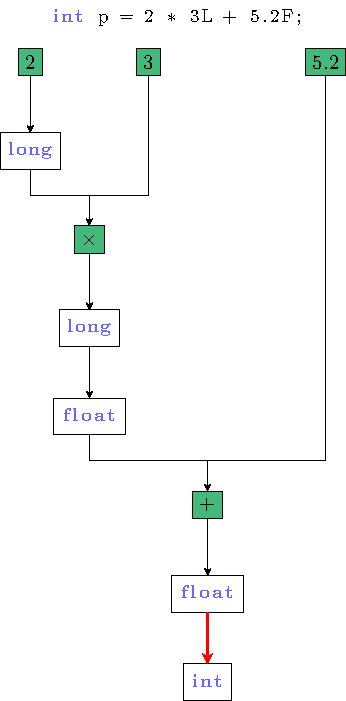
\includegraphics[height=7cm]{pics/conv.pdf}
\end{center}
\end{frame}

\begin{frame}
\frametitle{Autres conversions}
\begin{itemize}[<+->]
\item Opérateurs arithmétiques non définis pour \lstinline|short|, \lstinline|bool| et \lstinline|char|
\item Implicitement convertis en \lstinline|int| si présents 
	\begin{itemize}
	\item Caractères : dépend de l'encodage, de la machine, etc.
	\item Booléens : \lstinline|false| : $0$, \lstinline|true| : autre.
	\end{itemize}
\item Conversions non signées autorisées
	\begin{itemize}
	\item Parfois incohérent : que vaut $-5$ en non signé ?
	\end{itemize}
\item On peut effectuer des conversions explicites en faisant un cast
	\begin{itemize}
	\item En \texttt{C}, même syntaxe qu'en \java
	\item En \cpp, mécanisme de conversion dédié (cf. Ch. 8)
	\end{itemize}
%\item Chapitre 8 dédié aux conversions (implicites ou non)
\end{itemize}
\end{frame}

\begin{frame}[containsverbatim]
\frametitle{Exemple}
\begin{itemize}
\item Fichier \texttt{conv.c}
\item Même principe en \cpp
\end{itemize}
\begin{lstlisting}
int main()
{
	int i1 = 3;
	int i2 = 2.5;
	double d1 = i1;
	double d2 = 2.5f;

	unsigned u1 = i1;
	unsigned u2 = -1;

	printf("ints : %d %d\n", i1, i2);
	printf("floating point : %.2f %.2f\n", d1, d2);
	printf("unsigned : %u %u\n", u1, u2);

	printf("Sizeof int | float -- %lu %lu\n", sizeof(int), sizeof(double));

	printf("Sizeof 2 * 3L + 5.0 : %lu\n", sizeof(2 * 3L + 5.0));

	printf("%d\n", (0 == true));
	printf("%d\n", (1 == true));
	printf("%d\n", (2 == true));
}
\end{lstlisting}
\end{frame}

\begin{frame}
\frametitle{Les alias de type}
\begin{itemize}[<+->]
\item Nom référant un type défini précédemment
\item Utile pour abréger certains noms
\end{itemize}
\begin{exampleblock}<+->{Syntaxe en \texttt{C}}
	\begin{itemize}[<+->]
	\item \lstinline|typedef Type Alias;|
	\end{itemize}
\end{exampleblock}
\begin{itemize}[<+->]
\item Pratique pour abréger des noms de types longs
	\begin{itemize}
	\item \texttt{struct A -> A}
	\end{itemize}
\end{itemize}
\end{frame}

\begin{frame}[containsverbatim]
\frametitle{Exemple}
\begin{lstlisting}
struct point 
{
	double x, y;
};

typedef struct point point;

point p;
\end{lstlisting}
\begin{itemize}
\item Sans l'alias, on aurait dû écrire \texttt{struct point p;}
\end{itemize}
\end{frame}

\begin{frame}
\frametitle{Initialisation explicite}
\begin{itemize}[<+->]
\item Plusieurs types d'initialisation
	\begin{itemize}
	\item Initialisation scalaire
	\item Initialisation de tableaux (cf. Ch. 2)
	\item Initialisation de structures (cf. Ch. 4)
	\end{itemize}
\item Toutes les initialisation se font soit
	\begin{itemize}
	\item avec \texttt{=}
	\item avec \texttt{= \{ ... \}} (tableaux et structures)
	\end{itemize}
\item Des conversions, promotions et tronquages implicites sont possibles
\item En l'absence d'initialisation explicite, les valeurs par défaut dépendent du type d'allocation
	\begin{itemize}
	\item Cf. Ch. 5
	\end{itemize}
\end{itemize}
\end{frame}
%
\begin{frame}[containsverbatim]
\frametitle{Exemple}
\begin{itemize}
\item Fichier \texttt{init.c}
\end{itemize}
\begin{lstlisting}
int main()
{
    int i; //indeterminate
    int j = 2; 
	
    //unsigned char * p; //not a great idea
    //unsigned char * p = 2; //still up to no good

    unsigned char * p; //not a great idea
    *p = 3; 
    unsigned char * u = 2; //still up to no good
    *u = 3;
}
\end{lstlisting}
\end{frame}

%\begin{exampleblock}<+->{Exemple}
%	\begin{itemize}[<+->]
%	\item \lstinline|int i = 2.1; //ok|
%	\item \lstinline|int i(2.1); //ok|
%	\item \lstinline|int i|\texttt{\{ 2.1 \};} \lstinline|//ko|
%	\item \lstinline|int i|\texttt{\{ 2 \};} \lstinline|//ok|
%	\end{itemize}
%\end{exampleblock}
\end{document}
